% =============================================================================
% CAPÍTULO 5 — volta 2 (AGENTS.md §6): estabilidade e a sua quebra, como uma medida só.
%
% O fracasso que o abre, com número na mão: a estatística que estima o conjunto não anuncia o
% instante. O movimento do corte tem correlação de posto de +0,040 com os rompimentos dos 60
% dias seguintes; o nível do corte parece anunciar (+0,403) mas dá +0,414 num mundo que nunca
% muda — é sobreposição de janelas, e o controle é o que separa medida de aritmética.
%
% Medição: lab/experimentos/E06_estabilidade.ipynb. Figuras: figuras/E06_estabilidade_*.
% =============================================================================

\chapter{A estatística que não anuncia}
\label{cap:estabilidade}

\section{A conta que todo mundo faz}

Quem vigia um risco com uma linha tem dois trabalhos e um só instrumento. O primeiro é estimar:
que tamanho tem o dia ruim por aqui, e onde fica a linha que não se passa. O segundo é perceber
quando a resposta anterior deixou de valer. A prática corrente trata os dois separadamente
--- um filtro para o nível, um detector para a quebra ---, e o capítulo anterior já mostrou que o par de
um alarme custa caro.

A pergunta da volta é se esse par existe de verdade. Se a estatística que estima o conjunto for
a mesma que anuncia o instante, lida ao contrário, então calibrar as duas em separado é trabalho
dobrado sobre o mesmo objeto.

Vale escrever a conta mais simples possível, que é a que qualquer mesa faz sem pensar: se a
linha se moveu muito nos últimos sessenta dias, o mundo mudou, e o que vem depois deve romper a
linha mais vezes. É essa hipótese que a medição testa, e a resposta sai com um número.

\section{Três sinais e o que vem depois}

O palco é a mesma série de sempre, com \numEstabilidadeDias{} dias utilizáveis, o corte do
primeiro capítulo --- o décimo terceiro pior de \numCorteJanela{} --- e o bloco de
\numBlocoDias{} dias do segundo. Para cada dia, três sinais olhando para trás, e um alvo olhando
para frente: quantos rompimentos acontecem nos \numBlocoDias{} dias \emph{seguintes}. A média do
alvo é de \numEstabilidadeFuturoMedio{} rompimentos por bloco, e o pior bloco futuro tem
\numEstabilidadeFuturoPior.

Os três sinais são o \textbf{movimento do corte} (a estimativa se mexeu), a \textbf{contagem
recente} (o vigia do capítulo anterior) e o \textbf{nível do corte} (a própria estimativa, e a sua
versão dividida pela oscilação de agora).

A medida é a correlação de posto, e a escolha é deliberada: nada aqui supõe relação linear, e é
justamente na cauda que a relação deixa de ser linear.

\begin{table}[htbp]
  \centering
  \begin{tabular}{lrr}
    \hline
    sinal & correlação de posto & décimo mais baixo $\to$ mais alto \\
    \hline
    movimento do corte & \numEstabilidadeMovimentoPosto & \numEstabilidadeMovimentoPrimeiroDecimo\ $\to$ \numEstabilidadeMovimentoUltimoDecimo \\
    contagem recente & \numEstabilidadeContagemPosto & \numEstabilidadeContagemPrimeiroDecimo\ $\to$ \numEstabilidadeContagemUltimoDecimo \\
    nível do corte & \numEstabilidadeNivelPosto & \numEstabilidadeNivelPrimeiroDecimo\ $\to$ \numEstabilidadeNivelUltimoDecimo \\
    nível sobre a oscilação & \numEstabilidadeRelativoPosto & \numEstabilidadeRelativoPrimeiroDecimo\ $\to$ \numEstabilidadeRelativoUltimoDecimo \\
    \hline
  \end{tabular}
  \caption{Cada sinal olhando para trás, contra os rompimentos dos \numBlocoDias{} dias seguintes.
    A última coluna é a média do alvo no décimo mais baixo e no mais alto do sinal.}
  \label{tab:sinais}
\end{table}

A conta que a mesa faz está errada, e o erro é do tamanho do silêncio: o movimento do corte tem
posto \numEstabilidadeMovimentoPosto, e o seu perfil por décimo vai de
\numEstabilidadeMovimentoPrimeiroDecimo{} a \numEstabilidadeMovimentoUltimoDecimo{} sem ordem
nenhuma. A linha se mexer não diz nada sobre o que vem.

Quem tem informação é a contagem recente, que sobe de
\numEstabilidadeContagemPrimeiroDecimo{} para \numEstabilidadeContagemUltimoDecimo{} --- a
volatilidade tem memória, e isso é sabido \cite{engle1982autoregressive}. E há um terceiro número, maior que os outros dois: o
nível do corte caminha de \numEstabilidadeNivelPrimeiroDecimo{} para
\numEstabilidadeNivelUltimoDecimo, com posto \numEstabilidadeNivelPosto.

Seria uma descoberta boa, e é falsa. A seção seguinte é sobre como ela se desfaz.

\section{O controle que desfaz a leitura}

O nível do corte é parente próximo da oscilação do último ano --- a correlação entre os dois é
de \numEstabilidadeNivelComOscilacaoPosto, e o sinal é negativo porque corte fundo quer dizer
ano agitado. Sobra a dúvida óbvia: o nível anuncia alguma coisa, ou só repete a volatilidade que
todo mundo já vê? A resposta exigiu dois testes.

O primeiro foi dividir os dias em faixas de oscilação e medir o nível \emph{dentro} de cada
faixa, onde a oscilação é quase a mesma. O posto ficou em \numEstabilidadeFaixaBaixaNivelPosto{}
na faixa calma, \numEstabilidadeFaixaMediaNivelPosto{} na média e
\numEstabilidadeFaixaAltaNivelPosto{} na agitada. O nível sobrevive ao corte da oscilação. A contagem recente, medida nas mesmas faixas, dá
\numEstabilidadeFaixaBaixaContagemPosto{} na calma, \numEstabilidadeFaixaMediaContagemPosto{} na média e
\numEstabilidadeFaixaAltaContagemPosto{} na agitada: ela só aparece onde já há agitação para contar.

O segundo teste é o que decide, e é o mais barato de todos: um mundo em que nada muda. Retornos
sorteados, independentes, sempre a mesma lei, submetidos à mesma rotina. Nesse mundo não há nada
a anunciar, e a média do alvo é de \numEstabilidadeControleFuturoMedio{} rompimentos por bloco,
igual à do mercado. Aplicados os três sinais, o resultado é este.

\begin{table}[htbp]
  \centering
  \begin{tabular}{lrr}
    \hline
    sinal & no mercado & no mundo que nunca muda \\
    \hline
    movimento do corte & \numEstabilidadeMovimentoPosto & \numEstabilidadeControleMovimentoPosto \\
    contagem recente & \numEstabilidadeContagemPosto & \numEstabilidadeControleContagemPosto \\
    nível do corte & \numEstabilidadeNivelPosto & \numEstabilidadeControleNivelPosto \\
    \hline
  \end{tabular}
  \caption{Os mesmos três sinais nos dois mundos. No mundo em que nada muda não há o que
    anunciar, e ainda assim o nível do corte produz correlação.}
  \label{tab:controle}
\end{table}

O nível do corte dá \numEstabilidadeControleNivelPosto{} num mundo sorteado independente
--- mais do que os \numEstabilidadeNivelPosto{} que ele dá no mercado. Não há nada para
anunciar ali, e o número aparece.

O motivo é aritmético. O corte é o décimo terceiro pior dos \numCorteJanela{} dias anteriores,
e o alvo é contado com os cortes dos \numBlocoDias{} dias seguintes, cada um deles erguido numa
janela que carrega boa parte da mesma série de dias. As duas pontas se sobrepõem. Um corte fundo
quer dizer que o ano teve dias enormes, o que empurra a linha para longe e \emph{reduz} os
rompimentos que vêm; e é essa contabilidade, e não o mercado, que a correlação mede.

A lição vale além deste capítulo, e é a razão de ele existir: \textbf{uma medida sem o seu
controle é aritmética com nome de descoberta}. O mundo em que nada muda é o único instrumento
que separa as duas, e ele custa uma linha de código.

\begin{figure}[htbp]
  \centering
  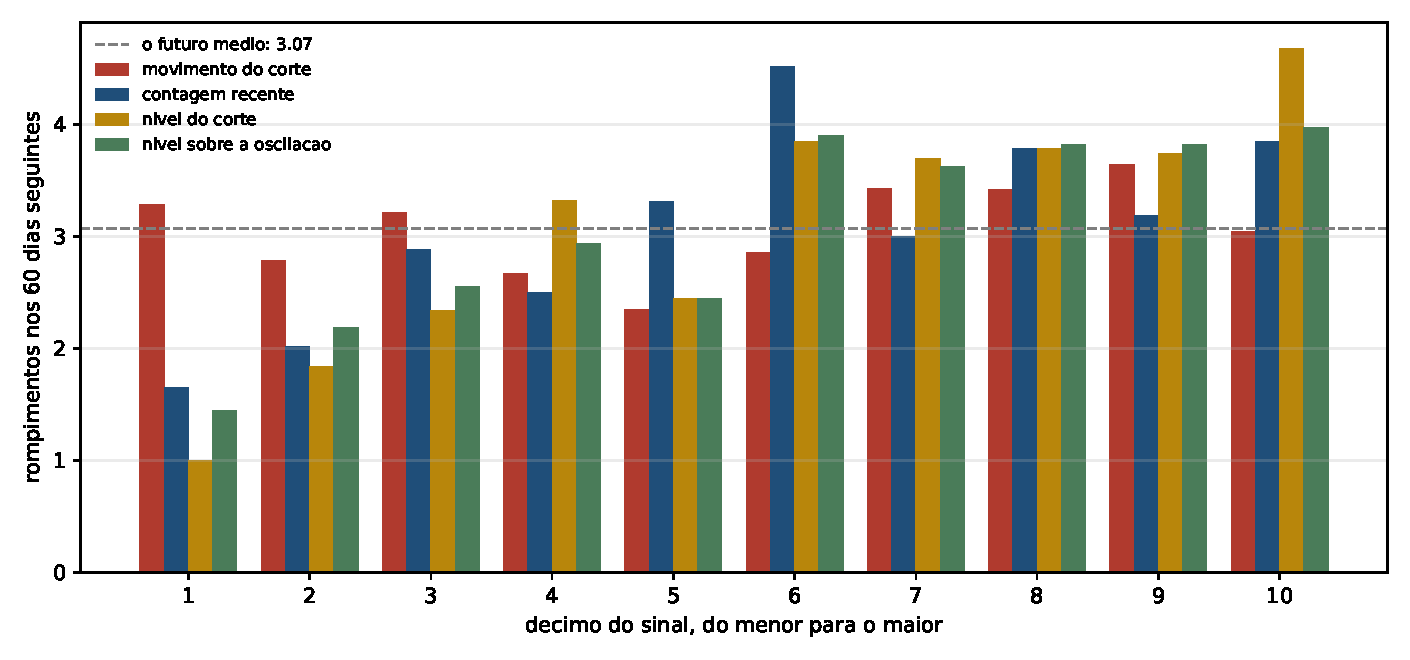
\includegraphics[width=\linewidth]{figuras/E06_estabilidade_1.pdf}
  \caption{O futuro médio em cada décimo dos quatro sinais, com a média geral como linha. Três dos quatro sobem; o do movimento do corte atravessa o gráfico de lado. A leitura é seguir uma cor de ponta a ponta: comparar décimos vizinhos perde a tendência, que é o que a figura mostra.}
  \label{fig:decimos}
\end{figure}

\begin{figure}[htbp]
  \centering
  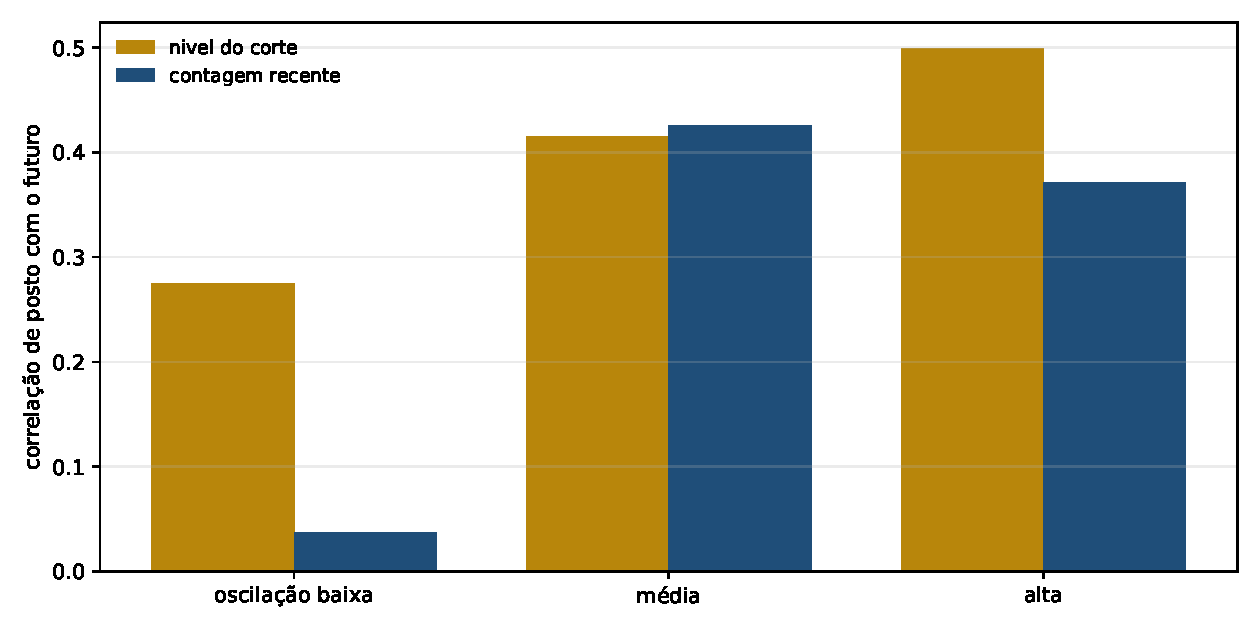
\includegraphics[width=\linewidth]{figuras/E06_estabilidade_2.pdf}
  \caption{O nível do corte e a contagem recente medidos dentro de três faixas de oscilação,
    onde a oscilação de agora é quase a mesma. O nível não desaparece ao dividir por ela. A barra quase ausente da contagem na faixa calma não é defeito: a contagem é cega justamente onde nada acontece.}
  \label{fig:faixas}
\end{figure}

\section{O que sobra}

Sobram dois números que o controle não explica, e os dois apontam para o mesmo lugar. A contagem
recente dá \numEstabilidadeContagemPosto{} no mercado contra
\numEstabilidadeControleContagemPosto{} no mundo parado: alguma coisa ali é do mundo, e é a
memória da oscilação que o capítulo anterior já usava. E a segunda série, o índice brasileiro, repete a
ordem: nível \numEstabilidadeSegundaPosto, contagem \numEstabilidadeSegundaContagemPosto,
movimento \numEstabilidadeSegundaMovimentoPosto.

A ordem é do dado, então, e não de um mercado. O movimento da estimativa fica em último nos dois.
O que a prática vigia --- a linha se mexeu, é hora de recalibrar --- é o único dos três sinais
que não vale nada, nem onde há o que prever nem onde não há.

\section{O que fica}

Fica a pergunta da volta, respondida pela metade e com o sinal trocado. A estatística que estima
o conjunto \emph{não} anuncia o instante em que ele deixa de valer; o que parecia anunciar era
sobreposição de janelas. Se as duas leituras são a mesma coisa, elas não são a mesma coisa
\emph{deste} jeito.

E fica a disciplina que o capítulo instalou, que vale para tudo o que vem depois: medir um sinal
exige medir o chão em que ele foi medido. Toda vez que um número deste livro parecer anunciar
alguma coisa, a pergunta passa a ser a mesma --- \emph{quanto disso sobra quando nada acontece?}
---, e o mundo que nunca muda é quem responde.

O fracasso seguinte não é de método, é de informação, e o próprio controle o deixou visível. Se
o corte é erguido numa janela e o alvo é contado em janelas que se sobrepõem a ela, a conta está
contaminada; mas tirar a sobreposição não é só cautela, é reconhecer que uma janela finita de
dias carrega uma quantidade finita de informação sobre a pergunta, e que essa quantidade pode
não dar para as duas leituras ao mesmo tempo. Quanto cabe num pedaço de passado, e a partir de
quando duas explicações diferentes ficam indistinguíveis nos mesmos dados, é a pergunta seguinte.
